
\documentclass[11pt,a4paper]{article}
 
\usepackage[utf8]{inputenc}
\usepackage[T1]{fontenc}
\usepackage{lmodern}
\usepackage[slovene,provide=*]{babel}
\usepackage[margin=2.2cm]{geometry}
\usepackage{amsmath}
\usepackage{enumitem}
\usepackage{booktabs}
\usepackage{caption}
\usepackage{pgfplots}
\pgfplotsset{compat=1.18}
\usepackage[colorlinks=true,linkcolor=black,urlcolor=blue]{hyperref}
 
\setlist[itemize]{topsep=2pt,itemsep=1pt,parsep=0pt}
\setlength{\parskip}{2pt}
 
\pagestyle{empty}
 
\begin{document}
 
\begin{center}
{\Large\bfseries Eksponentna rast prebivalstva: od bakterij do Zemlje}\\[4pt]
\normalsize Seminarska naloga pri matematiki\\
Ime in priimek dijaka, 3.~letnik \quad$\vert$\quad Šolski center Krško--Sevnica\\
Mentor: ime priimek \quad$\vert$\quad Krško, 2026
\end{center}
 
\vspace{4pt}
\noindent\textbf{Snov:} eksponentna funkcija (poglavje 16 -- Matematika na maturi, cilji)
 
\section*{Uvod}
 
Leta 1798 je angleški duhovnik in ekonomist \textbf{Thomas Robert Malthus} objavil delo \textit{An Essay on the Principle of Population}, v katerem je opozoril na preprosto, a nemirujočo idejo: če prebivalstvo raste \emph{eksponentno}, viri, ki ga hranijo, pa le \emph{linearno}, se prej ali slej zgodi kriza. Vprašanje, ali se stvari v naravi in pri človeku res množijo eksponentno -- in kaj to pomeni za prihodnost --, je aktualno še danes, ko govorimo o prenaseljenosti, podnebnih spremembah in omejenih virih.
 
V tej nalogi bom pokazal(a), kako eksponentna funkcija opiše rast populacij v naravi, jo uporabil(a) za oceno rasti svetovnega prebivalstva in preveril(a), ali taka napoved drži tudi na dolgi rok -- ter na koncu predstavil(a) Malthusovo teorijo in njene meje.
 
\section*{Jedro}
 
\subsection*{Matematični model}
 
Populacijo, ki raste s stalno stopnjo rasti $r$ na časovno enoto, opišemo z eksponentno funkcijo
\[
N(t) = N_0 \cdot (1+r)^t \qquad \text{oz.\ zvezno} \qquad N(t) = N_0 \cdot e^{rt},
\]
kjer je $N_0$ začetno število osebkov, $t$ pa preteklo časovno obdobje. Pogosto nas zanima \textbf{podvojitveni čas} $t_2$ -- čas, v katerem se populacija podvoji:
\[
N_0\cdot e^{r t_2} = 2N_0 \;\;\Rightarrow\;\; t_2 = \frac{\ln 2}{r} \approx \frac{0{,}693}{r}.
\]
 
\subsection*{Primeri iz narave}
 
\begin{itemize}
  \item \textbf{Bakterije.} Bakterija \textit{E.\ coli} se v ugodnih razmerah podvoji približno vsakih 20 minut. Iz ene same bakterije bi po 8 urah (480 minutah, torej $480/20=24$ podvojitvah) nastalo
  \[
  N = 1 \cdot 2^{24} \approx 16{,}8 \text{ milijona bakterij.}
  \]
  Brez omejitev (prostor, hrana) bi taka kultura v enem samem dnevu presegla maso Zemlje -- kar seveda pokaže, da v resnici prej ali slej nekaj rast ustavi.
  \item \textbf{Zajci v Avstraliji.} Leta 1859 je bilo v Avstralijo prineseno le 24 divjih zajcev. Ker tam niso imeli naravnih sovražnikov, se je populacija v manj kot desetih letih razrasla na več deset milijonov -- eden najbolj znanih primerov nemotene eksponentne rasti v naravi.
  \item \textbf{Cvetenje alg.} Ob obilju hranil (npr.\ dušika iz gnojil, ki odteče v jezero) se alge razmnožujejo eksponentno in v nekaj dneh prekrijejo celotno vodno površino, kar zaduši ostalo življenje v vodi.
\end{itemize}
 
\subsection*{Rast svetovnega prebivalstva}
 
Svetovno prebivalstvo je v zadnjih dveh stoletjih naraščalo takole: 1 milijarda (1804), 2 mrd (1927), 3 mrd (1960), 4 mrd (1974), 5 mrd (1987), 6 mrd (1999), 7 mrd (2011), 8 mrd (2022). Med letoma 1960 in 1999 se je prebivalstvo natanko podvojilo (iz 3 na 6 mrd) v 39 letih, kar pomeni letno stopnjo rasti
\[
r = \frac{\ln 2}{39} \approx 0{,}0178 = 1{,}78\,\%.
\]
 
Kaj pa napoved? Če bi to stopnjo ($r\approx 1\,\%$, kolikor znaša ocenjena \emph{trenutna} globalna rast) preprosto uporabili tudi za prihodnost, bi za leto 2100 (78 let po letu 2022, ko je bilo 8 mrd ljudi) dobili
\[
N(2100) = 8 \cdot e^{0{,}01 \cdot 78} \approx 8 \cdot 2{,}18 \approx 17{,}4 \text{ milijarde}.
\]
Združeni narodi (\textit{World Population Prospects 2022}) pa za leto 2100 napovedujejo le okoli \textbf{10,4 milijarde} -- torej precej manj. Slika~\ref{fig:napoved} to razliko lepo pokaže.
 
\begin{center}
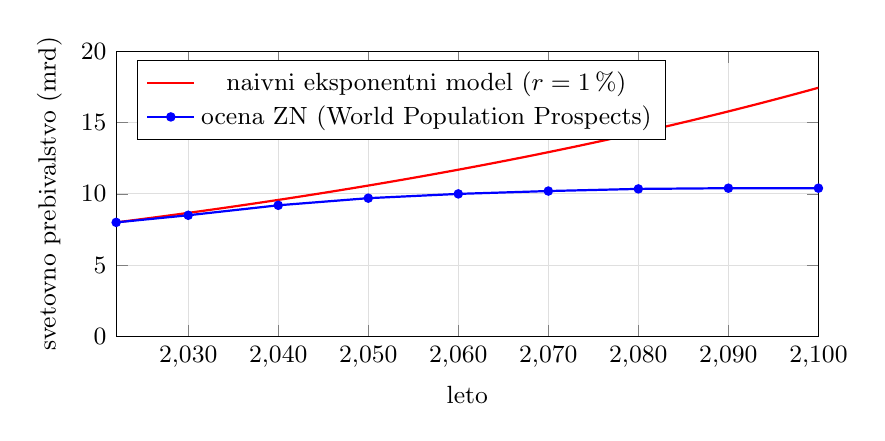
\begin{tikzpicture}
\begin{axis}[
  width=10.5cm, height=5.2cm,
  xlabel={leto}, ylabel={svetovno prebivalstvo (mrd)},
  xmin=2022, xmax=2100, ymin=0, ymax=20,
  legend pos=north west, legend style={font=\small},
  label style={font=\small}, tick label style={font=\small},
  grid=major, grid style={gray!25}
]
\addplot[domain=2022:2100, samples=60, thick, red] {8*exp(0.01*(x-2022))};
\addlegendentry{naivni eksponentni model ($r=1\,\%$)}
\addplot[thick, blue, mark=*, mark size=1.3pt] coordinates {
  (2022,8.0) (2030,8.5) (2040,9.2) (2050,9.7) (2060,10.0)
  (2070,10.2) (2080,10.35) (2090,10.4) (2100,10.4)
};
\addlegendentry{ocena ZN (World Population Prospects)}
\end{axis}
\end{tikzpicture}
\captionof{figure}{Primerjava naivnega eksponentnega modela z oceno Združenih narodov.}
\label{fig:napoved}
\end{center}
 
Razlog za odstopanje je, da stopnja rasti $r$ pri ljudeh \emph{ni} konstantna, kot smo predpostavili: z gospodarskim razvojem, izobrazbo (predvsem žensk) in dostopnostjo kontracepcije se rodnost zniža -- pojav imenujemo \textbf{demografski prehod}. Eksponentni model je torej dober približek na kratek rok, na dolgi rok pa ga je treba nadomestiti z modelom, kjer se $r$ s časom zmanjšuje (npr.\ z logistično funkcijo, ki pa presega gimnazijsko snov).
 
\subsection*{Malthusova past}
 
Malthus je trdil, da prebivalstvo raste \textbf{geometrijsko} (eksponentno): $1,2,4,8,16,\dots$, pridelava hrane pa le \textbf{aritmetično} (linearno): $1,2,3,4,5,\dots$. Tabela~\ref{tab:malthus} to ponazori na sedmih ,,generacijah``.
 
\begin{center}
\begin{tabular}{cccc}
\toprule
generacija $n$ & prebivalstvo $P_n=2^n$ & hrana $F_n=n+1$ & razmerje $P_n/F_n$ \\
\midrule
0 & 1  & 1 & 1{,}0 \\
1 & 2  & 2 & 1{,}0 \\
2 & 4  & 3 & 1{,}3 \\
3 & 8  & 4 & 2{,}0 \\
4 & 16 & 5 & 3{,}2 \\
5 & 32 & 6 & 5{,}3 \\
6 & 64 & 7 & 9{,}1 \\
\bottomrule
\end{tabular}
\captionof{table}{Geometrijska rast prebivalstva proti aritmetični rasti hrane.}
\label{tab:malthus}
\end{center}
 
Razmerje $P_n/F_n$ narašča vse hitreje -- ravno to je ,,Malthusova past``: prebivalstvo prej ali slej preraste svoje vire, kar po Malthusu vodi v lakoto, bolezni ali vojne, ki populacijo spet zmanjšajo.
 
\section*{Zaključek}
 
Eksponentna funkcija zelo dobro opiše rast v idealnih razmerah -- pri bakterijah, pri zajcih brez plenilcev, pri algah ob obilju hranil, pa tudi pri človeku na krajših časovnih obdobjih (npr.\ 1960--1999). Na dolgi rok pa noben resničen sistem ne raste eksponentno v nedogled, ker mu prej ali slej zmanjka prostora, hrane ali drugih virov -- kar so pokazali tako izračun za bakterijsko kulturo kot primerjava z napovedjo ZN za leto 2100.
 
Malthus je s tem, ko je opozoril na neskladje med (eksponentno) rastjo prebivalstva in (linearno) rastjo virov, postavil pomembno vprašanje, ki je še danes v ospredju razprav o trajnostnem razvoju. Ni pa predvidel, kako močno lahko tehnološki napredek (npr.\ ,,zelena revolucija`` v kmetijstvu 20.\ stoletja) poveča razpoložljive vire in s tem odloži ali omili ,,past``. Sama Malthusova past se torej (še) ni uresničila v takšni obliki, kot jo je opisal, njegov temeljni matematični vpogled -- da eksponentna rast prej ali slej trči ob omejene, kvečjemu linearno rastoče vire -- pa ostaja veljaven in uporaben tudi zunaj demografije, na primer pri porabi naravnih virov ali širjenju epidemij.
 
\section*{Literatura}
 
\begin{itemize}
  \item Malthus, T.\,R. (1798). \textit{An Essay on the Principle of Population}. London: J.\ Johnson.
  \item United Nations, Department of Economic and Social Affairs, Population Division (2022). \textit{World Population Prospects 2022: Summary of Results.}
  \item Our World in Data -- \url{https://ourworldindata.org/world-population-growth} (dostop: 2026).
  \item Učbenik za matematiko, 3.\ letnik gimnazije -- poglavje o eksponentni funkciji.
\end{itemize}
 
\end{document}
 
Downloaded seminarske-naloge-matematika.tex Show in Explorer